\documentclass[../thesis.tex]{subfiles}
  \begin{document}
\chapter{Introduction}\label{cap:introduction}

\section{Background and motivation}
Improving the way an operator can interact with a robot is a hard challenge in the field of \acrfull{HRI}. Nowadays, robots are everywhere, and the control of their movements and actions is usually done through a joystick or a dashboard in case of very complicated tasks.\\
The idea of using the operator's body to interact with a robot is not a new one, but it brings several challenges when trying to implement it. A possible solution would be to use computer vision and machine learning techniques. In recent years, the computational power of processors and the ability to deploy \acrfull{ML} models on cheaper and smaller devices have paved the way to interact with computers and robots in a way previously unfeasible.

\section{Problem statement}
The main idea of the project is to improve the interaction between human and robots through computer vision and \acrshort{ML} to detect a set of hand gestures in real time and convey to a robot the action to take in response to the gesture. In this way, the operator can use the expressive power of his/her hands and their immediacy to communicate with the robot. Furthermore, by implementing this concept as an interface using the \acrfull{ROS} framework, we will no longer have to worry about which robot we want to manage in the future; all that is required is that it receives specified messages in order to function. An example of the idea we want to implement is the one in~\ref{fig:systemArchitecture}.

\begin{figure}[H]
  \centering
  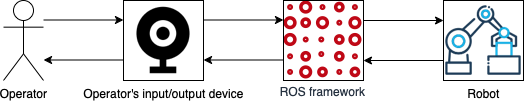
\includegraphics[width=0.7\columnwidth]{thesis/images/systemArchitecture.png}
  \caption{Example of system architecture.}
  \label{fig:systemArchitecture}
\end{figure}

A warehouse environment has been chosen to test the system because since 2011 Amazon started using robots inside its warehouses, and nowadays, the number of warehouses that use robots to carry products is fastly growing~\cite{paper:bogue2016}. Anyway, a modular system would allow to easily change the actions performed by the robot in response to a gesture or change the gestures the system can recognize.\\
The system designed should be able to:
\begin{itemize}
    \item recognize a set of hand gesture;
    \item communicate with a robot through the \acrshort{ROS} framework;
    \item learn new gestures from the user;
    \item record some \glsfirstplural{macro}, save and execute them;
    \item allow the user to change its behaviour in response to a gesture.
\end{itemize}
To complete all of these tasks, I combed the literature for information on the state of the art of the \acrshort{HRI}, its evaluation methods, and the best way to perform a hand gesture recognition task.

\section{Related works}
TBD

\section{Organization}\label{s:organization}
This document is organized as follow:
\begin{description}
    \item[{\hyperref[cap:theory]{Chapter two}}] describes the background I obtained studying the literature about \acrlong{HRI} and hand gestures recognition.
    \item[{\hyperref[cap:methods]{Chapter three}}] describes the technologies and tools used to implement the solution proposed and why they have been chosen to fulfill the requirements. Moreover, the the design process that led to the solution proposed is described. In particular, it is focused on the implementation of the system composed by the hand gesture recognizer and a robot employed in a warehouse (i.e. a storage and retrieval robot).
    \item[{\hyperref[cap:results]{Chapter four}}] describes ...
    \item[{\hyperref[cap:discussion]{Chapter five}}] describes ...
    \item[{\hyperref[cap:conclusion]{Chapter six}}] describes ...
\end{description}

\end{document}
